% Seminar Thesis Template - Chair for High-Performance Computing
% Note: If you write your thesis in German, then change the babel package include
%       to "ngerman".
%
% TODOs:
% 1. Configure the seminar thesis options (title, author, ...) in "my_config.tex".
% 2. If the language of your thesis is not English: Change the option in the babel
%    package import to "ngerman". (see below)
% 3. (Optional) You might want to switch the BibLaTeX backend from "bibtex" to "biber".
%
\documentclass[10pt,          % font size
               a4paper,       % page layout
               % twocolumn,     % two-column format
               DIV=14,        % page margins
               BCOR=8mm,      % binding correction for two-sided prints
               twoside        % for two-sided prints
              ]{scrartcl}

% TODO: Set language here
\usepackage[english]{babel}   % change to "ngerman" if you write your thesis in German

\usepackage{hpcseminar}
\usepackage[utf8]{inputenc}   % UTF-8 encoding (for umlauts etc.)
\usepackage[T1]{fontenc}      % correct hyphenation
\usepackage{csquotes}         % correct quotation marks
\usepackage{lmodern}          % Computer Modern fonts
\usepackage{microtype}        % better typesetting results (avoids underfull / overfull hboxes)
\usepackage{graphicx}         % adding graphics
\usepackage{units}            % typesetting units, e.g. \unit[10]{MB} and \unitfrac[100]{Mbit}{s}
\usepackage{booktabs}         % publication quality tables
% \usepackage{siunitx}         % alternative (more features) unit typesetting package


% BibLaTeX settings
\usepackage[backend=bibtex, style=numeric, maxcitenames=2, natbib=true]{biblatex}
\addbibresource{literature}

%% TODO: Put your own includes in "includes.tex"
% Platz f\"{u}r eigene Erweiterungen und Definitionen

%\usepackage{XYZ}
%\newcommand{\hi}{Hallo}
\usepackage{graphicx}
\usepackage{hyperref}
\usepackage{listings}
\usepackage{xcolor}
\usepackage{amsmath}
\usepackage[capposition=top]{floatrow}


\begin{document}

%% TODO: Configure details in configs.tex
%% Ein paar wichtige Details konfigurieren
%%----------------------------------------
\title{Automatic Transformation of Blocking into Non-Blocking MPI Communication}
\author{Khoa Phuc Viet Nguyen}
\supervisor{Isa Thärigen, M. Sc.}
\semester{Summer Term 2023}
\keywords{MPI, Blocking/Non-blocking Operations, Communication-Computation Overlap, Automatic Transformation, Code Generation}
% \setcounter{tocdepth}{5}
\setcounter{secnumdepth}{4}
% \bibliographystyle{ieeetr}
\definecolor{greenComment}{rgb}{0,0.6,0}
\lstset{
        language=c,
        basicstyle=\ttfamily,
        columns=fullflexible,
        frame=single,
        numbers=left,
        breaklines=true,
        keywordstyle=\color{blue},
        commentstyle=\color{greenComment}\ttfamily,
        stringstyle=\color{red},
        rulecolor=\color{black},
        postbreak=\mbox{\textcolor{red}{$\hookrightarrow$}\space},
        emph={int,char,double,float,unsigned,void,bool},
        morekeywords={sem_t, NULL, pid_t, uint32_t},
        % xleftmargin=2em,
        % frame=single,
        % framexleftmargin=1.5em,
        literate= %German
        {Ö}{{\"O}}1
        {Ä}{{\"A}}1
        {Ü}{{\"U}}1
        {ß}{{\ss}}2
        {ü}{{\"u}}1
        {ä}{{\"a}}1
        {ö}{{\"o}}1
      }

% Generate title
\maketitle

% Abstract
% TODO: Write your abstract in "abstract.tex"
\begin{abstract}


% Print out keywords
\noindent\keywordsline
\end{abstract}

% Chapters are included here
% TODO: Add your chapters in "chapters.tex"
% Sections / Chapters are included here
% Include your own sections / chapters if needed
\noindent
In parallel applications, even when there is ample parallelism and effective load balancing, a common challenge arises that negatively impacts performance. Processes idling while waiting for remote data from other processes leads to a reduced efficiency of the program. Network latencies and synchronization among processes are two significant factors which can lead to these communication delays. To address this problem, one potential approach is to reduce the influence of communication costs by overlapping them with local computational tasks, effectively concealing the additional time and resources required for communication.
While manual transformation is possible, it is often complex and prone to errors. To address this issue, several frameworks and tools have been developed to automate the transformation process. This paper aims to gather the key contributions related to the overlapping of computation and communication in MPI communications. Additionally, it provides a technical explanation of how such communications can be automatically transformed using specific frameworks and tools.

\section{Introduction}
MPI \cite{noauthor_mpi_nodate} library is usually used for parallel high-performance computing that includes a wide variety of point-to-point and group communication operations. MPI enables efficient communication by eliminating the need for memory-to-memory copying, enabling computation and communication to occur simultaneously, and facilitating offloading to communication coprocessors, if they are present. 
In distributed computing scenarios, communication plays a crucially significant role, encompassing collaborative multimedia applications, parallel computing across workstation clusters, and high-performance computing over computational grids. By effectively optimizing communication mechanisms, these systems can derive substantial benefits and achieve enhanced performance levels. 

Enhancing basic communication performance can be accomplished through the utilization of advanced communication hardware and specialized middleware. This approach aims to reduce latency and enhance bandwidth. However, focusing solely on bandwidth and latency has its limitations when it comes to improving overall application performance. To overcome these limitations, strategies that integrate computation and communication have been developed. By simultaneously performing communication and computation, these approaches aim to hide the costs associated with latency. Achieving true overlap and reaping the associated performance benefits requires support from both hardware and middleware, which can sometimes place significant demands on communication hardware. To harness this parallelism effectively, programmers must have access to specific non-blocking semantics. \cite{hoefler_leveraging_2008}\\
For example, for applications using collective operations, a simple textual replacement of blocking to non-blocking communication does not suffice to derive any significant benefit. To attain advantages of non-blocking features, developers have to identify independent parts in the code that can be interposed between a collective call and WAIT/ TEST (compatibly across the group of the MPI communicator) in order to expose computation that might overlap with the non-blocking collective.\\
Previous work \cite{calland_tiling_1999}\cite{danalis_transformations_2005}\cite{baude_optimizing_2001} presents  the techniques and schemas to manually transform blocking to non-blocking communication. Torsten Hoefler \cite{hoefler_leveraging_2008} et al suggest possibilities to leverage performance for manual transformation. It requires some techniques such as loop tiling, loop indexing and loop distribution and tuning parameters which need to be done manually and require deep understanding about the system in order to maximize overlapping to achieve better overlapping. Transforming applications manually in such way requires a lot of effort to tune the parameters and is potentially error-prone and time-consuming.\cite{sancho_mpi_2006}

In order to simplify the developer's work and to help ensure periodic introduction of new library features seamlessly into these applications, the goal of this work is to automate the process of changing operations from blocking to non-blocking as well as to the expected corresponding near-future persistent variants thereof.

In this paper, I present compiler-based tools and frameworks aimed at automating the transformation of user programs that rely on blocking operations into more efficient non-blocking variants. By automatically implementing these transformations, these transformations, the goal is to achieve enhanced performance in parallel computing scenarios.

In Section 2, we provide a comprehensive overview of standard MPI communications, contextualizing the need for automatic transformations for our proposed transformations. Additionally, we briefly outline the key principles underlying the transformation approach. Building upon this foundation, Section 3 focuses on exploring in detail and the frameworks and Petal tools employed, showcasing their advanced capabilities in automatically transforming the code.
To demonstrate the effectiveness of our these tools, Section 4 presents a specific case study  where the presented transformations were successfully applied to a parallel code. By effectively overlapping communication and computation, this transformed code achieved performance gains.

Subsequent sections delve into important areas of discussion, including the identification of potential avenues for future research, an examination of the limitations inherent in the presented tools and frameworks, and finally, the presentation of our conclusive findings.

\section{MPI Communication}
The Message Passing Interface (MPI)  is a commonly employed standard in high-performance computing (HPC) for programming distributed memory systems. 
Instead of offering an implementation, MPI serves as an application programming interface (API), comprising functions, constants, and expected behaviors. 
Various vendors offer their own implementations of this API, such as Open MPI.\\
MPI operations consist of a sequential sequence of steps: initialization, starting, completion, and freeing. 
These actions can be carried out in one or more MPI procedures and are carried out by the MPI library. The many forms of communication are thoroughly explained in the paragraphs that follow.\\

\subsection{Point-to-point Communications and Collective Communication.}
In general, MPI offers three different communication paradigms determining how processes communicate with the others: point-to-point, one-sided, and collective communication.
Point-to-point (P2P) communication is the simplest form, as it only involves exactly two processes, which both actively take part in the communication. 
One process sends a message (e.g., using \texttt{MPI\_Send}), which the receive process receives with a corresponding receive call (e.g., \texttt{MPI\_Recv}).
One-sided communication also involves two processes, but only one of them has to actively take part in the communication. This work does not focus on one-sided communication, so it will not be discussed in detail.\\
Finally, collective communication entails the exchange of messages among multiple processes. 
For instance, an individual process can broadcast a message to all other processes within the same group, utilizing the \texttt{MPI\_Bcast} function. 
Every collective communication can be implemented through peer-to-peer communication calls.

\subsection{Blocking and non-blocking communication.}
In blocking communication, four steps (initialization, starting, completion and freeing) are combined into single one and must be performed sequentially without interrupt. 
A state transition diagram for blocking operations is shown in \autoref{fig:mpi_blocking}.
\begin{figure}[h!]
    \centering
    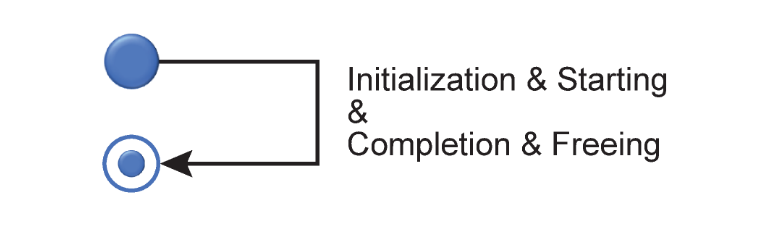
\includegraphics[width=0.5\textwidth]{pictures/mpi_blocking.png}
    \caption{State transition diagram for blocking operations. \cite{noauthor_mpi_nodate}}
    \label{fig:mpi_blocking}    
\end{figure}

Blocking means that the MPI primitive waits until the message buffer containing the data being sent/received is safe to be used again by the calling process. 
Only then is control returned to the caller.
On send, actual implementations of \texttt{MPI\_Send} may either block until all data has been transmitted or copy the data to an intermediate internal buffer. 
The use of blocking primitives may be prone to deadlocks, if programmers do not carefully consider send and receive order.
\texttt{MPI\_Isend} and \texttt{MPI\_Irecv} are non-blocking message communication. 
Compared to \texttt{MPI\_Send}'s arguments, \texttt{MPI\_Isend} adds an additional argument for a request handle. The handle is used in calls to \texttt{MPI\_Wait} to identify which send to wait for.\\
The non-blocking process combines the initialization and starting phases into a single procedure call that does not block, while the completion and freeing stages are handled in a separate procedure call, which can be either blocking or non-blocking.
A state transition diagram for non-blocking operations is shown in \autoref{fig:mpi_non_blocking}.\\
\begin{figure}[h!]
    \centering
    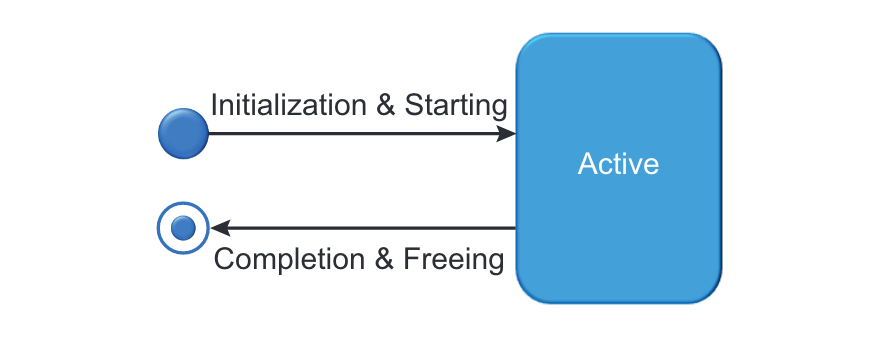
\includegraphics[width=0.5\textwidth]{pictures/mpi_non-blocking.png}
    \caption{State transition diagram for non-blocking operations. \cite{noauthor_mpi_nodate}}
    \label{fig:mpi_non_blocking}
\end{figure}
Non-blocking calls return immediately after initiating the communication and the user thread can execute more operations, eventually followed by a completion operation (a wait or test) on the request. The communication is considered complete after a successful call to \texttt{MPI\_Wait} (or \texttt{MPI\_Test}, etc.). 
Non-blocking is used to help promote overlap communication and computation, resulting in communicating cost hiding and yielding overall better performance on systems that support it. To avoid tampering with the data, programmers must ensure that the message data is not modified before the communication is completed.

\section{Automatic Transformation of MPI Code}

Petal is a transformation tool, which is a rejuvenation tool, implemented by Pirkelbauer et al. \cite{pirkelbauer_source_2010} which is built upon the ROSE source-to-source infrastructure. 
By utilizing the analysis APIs provided by ROSE, Petal enables the conversion of blocking collective primitives and point-to-point communication into their non-blocking equivalents. 
This transformation unveils greater opportunities for overlap between computation and communication, while also incorporating persistent operations wherever feasible to minimize the overhead associated with frequent communication with partner nodes.\\

\subsection{ROSE compiler infrastructure}
The ROSE \cite{quinlan_rose_2023} source-to-source translation infrastructure is under active development at the Lawrence Livermore National Laboratory (LLNL). ROSE provides front ends for many languages, including C/C++, FORTRAN 77/95/2003, and Java. ROSE also supports several parallel extensions, such as OpenMP, MPI and CUDA. ROSE generates an Abstract Syntax Tree (AST) for the source code. The ASTs are uniformly built for all input languages. ROSE offers many specific analyses (e.g., pointer alias analysis) and makes these available through an API. Users can write their own analyses by utilizing frameworks that ROSE provides. Rose also includes several program analyses, including control-flow and data-flow analyses and data dependence and system dependence analyses. Rose has developed a wide range of transformations and optimizations via manipulating AST, including partial redundancy elimination, constant folding, inlining, outlining, automatic parallelization, and various loop transformations. ROSE comprises the autoPar tool, which is an implementation of automatic parallelization using OpenMP. It can automatically insert OpenMP 3.0 directives into serial C/C++ codes.

\begin{figure}[h!]
    \centering
    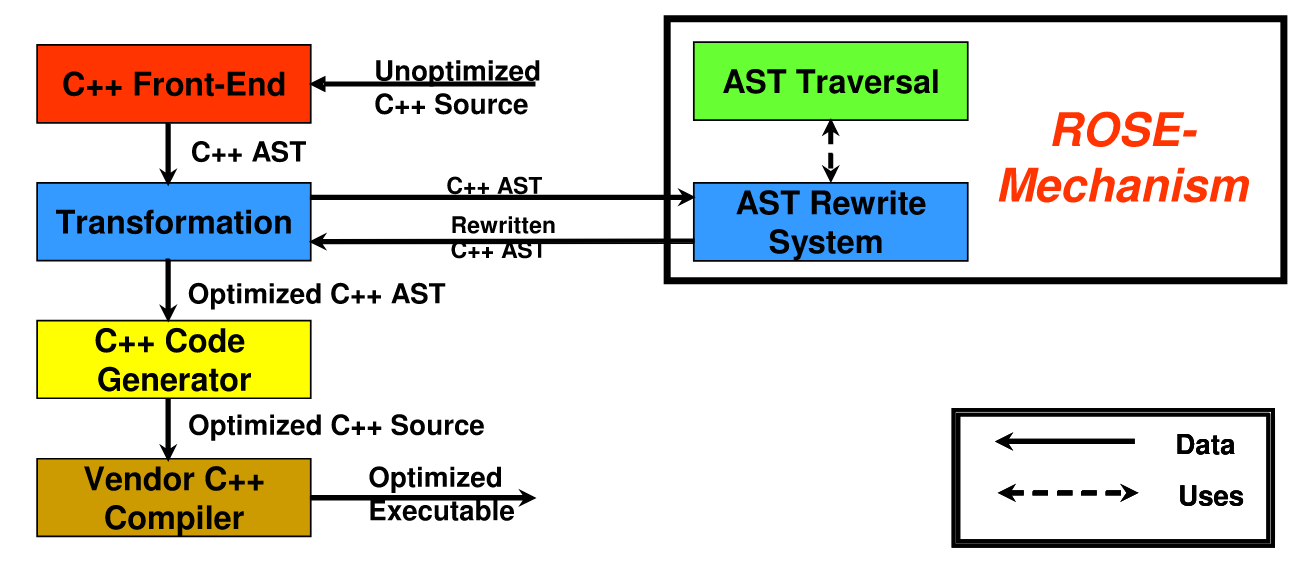
\includegraphics[width=0.7\textwidth]{pictures/rose.png}
    \caption{The ROSE compiler infrastructure.}
    \label{fig:rose}
\end{figure}
The flow diagram in \autoref{fig:rose}  reflects the complete approach, transforming unoptimized C++ code based on user defined abstractions into highly optimized code.
Using the code's Abstract Syntax Tree (AST) representation and leveraging the static analysis capabilities of the ROSE libraries, one can analyze the code and identify opportunities for improvement. This entails identifying particular code style elements, introducing new code segments, modifying or removing existing code, all while preserving the original code's intended semantics.

\begin{figure}[!h]
    \centering
    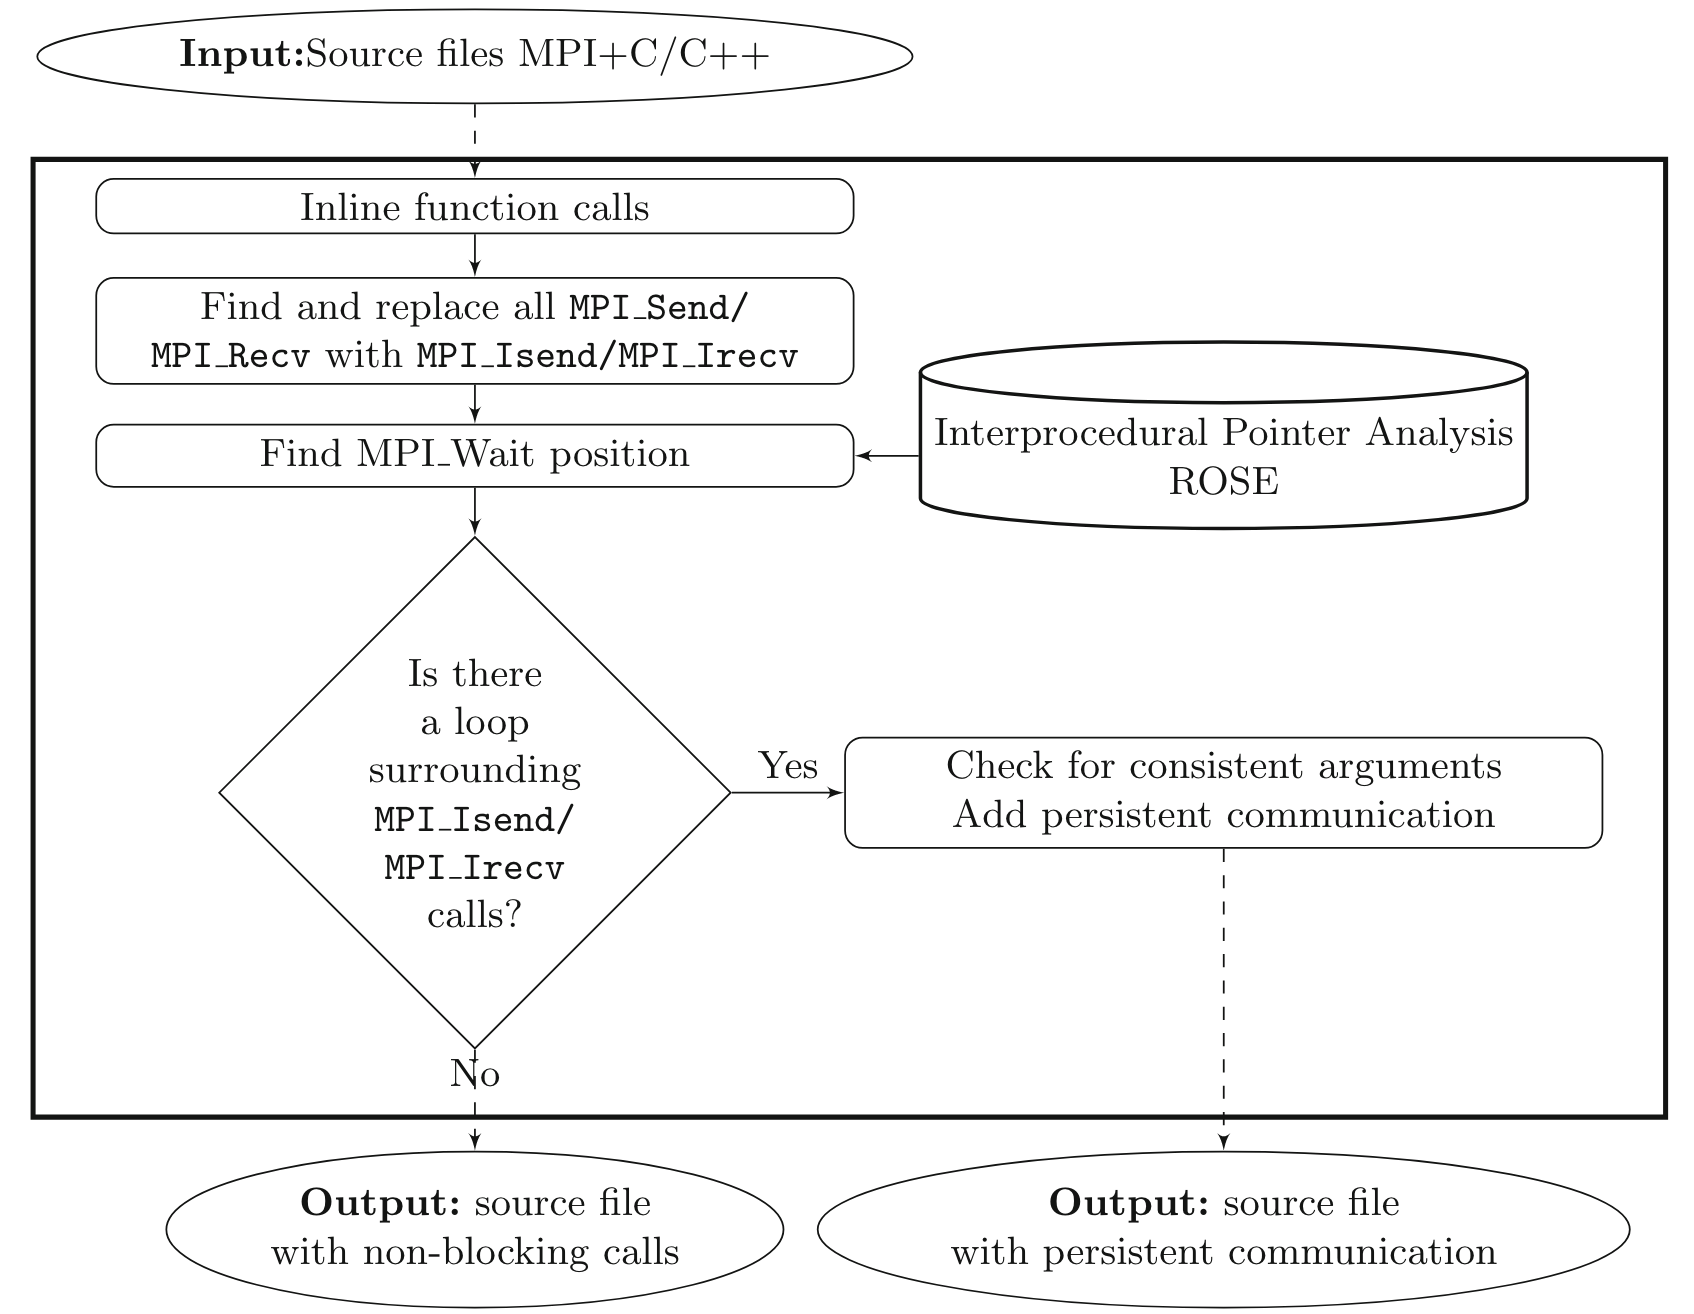
\includegraphics[width=0.7\textwidth]{pictures/petal_p2p_workflow.png}
    \caption{The Petal transformation framework for poin-to-point communications. \cite{ahmed_petal_2016}}
    \label{fig:petal-p2p-workflow}
\end{figure}
An overview of the transformation framework for point-to-point operations is shown in \autoref{fig:petal-p2p-workflow}. 
With transformations for collective operations, after inlining functions, Petal will perform some addition analysis. Transformation framework for colective operations is illustrated in \autoref{fig:petal-collective-workflow}. Petal will count the number of calls to blocking collectives within each block. 
The count is needed to allocate the maximum number of \texttt{MPI\_Request} and status objects that are needed, and reuse the same request for communications on mutually exclusive paths. 
If the function implementation is available, the function calls are then inlined. After being inlined, ROSE's query and builder libraries are used to locate blocking calls, replace them with non-blocking ones, and determine where to put \texttt{MPI\_Wait()} calls in their place. 
These non-blocking calls are replaced with persistent communication operations if any or all of them are invoked again with the same parameters. 
Petal ultimately creates a new source code, utilizing either persistent communications (which are always non-blocking) or non-blocking communications.  Following this strategy is based on the need to increase communication and computation overlap without sacrificing the original application's semantics.
\subsubsection{Blocking to Non-blocking Transformation}
To provide proper access to message buffers, Petal permits the replacement of the blocked function calls \texttt{MPI\_Send} and \texttt{MPI\_Recv} with their corresponding \texttt{MPI\_Isend} and \texttt{MPI\_Irecv}. 
In order to ensure the safety of the data, Petal inserts \texttt{MPI\_Wait} before any operations that access the message buffer. \cite{ahmed_petal_2016}

\subsubsection{Transformation of Point-to-Point Communication}

The basic point-to-point communication operations are send and receive with corresponding blocking function  \texttt{MPI\_Send} and \texttt{MPI\_Recv} in C binding. 
Calling \texttt{MPI\_Send/MPI\_Recv} is in effect the same as calling \texttt{MPI\_Isend/MPI\_Irecv} immediately followed by \texttt{MPI\_Wait()}.

Three variables are constructed to replace each blocking call with its matching non-blocking alternative. 
Two of these variables serve as handlers for \texttt{MPI\_Request} and \texttt{MPI\_Status}. The third variable is a flag added to ensure the \texttt{MPI\_Wait} of the corresponding non-blocking call is correctly executed. 
Instead of each blocking call, \texttt{MPI\_Isend/MPI\_Irecv} are used instead. The next step is to identify the subsequent statements, extract the variables utilized within those statements, and perform pointer analysis to look for any potential aliasing between the variables at hand and the message buffer. 
Petal recognizes probable update activities while dealing with send operations, such as variables that occur on the left-hand side of assignments. 
Petals use the pointer alias analysis from ROSE infrastructure to check the possibilities for an update could modify some data.

Petal shifts the \texttt{MPI\_Wait} operation downwards along the forward control flow edges, ensuring the safety of operations concerning MPI operations and buffer access. 
To ensure code correctness, any write made to a message buffer utilized in a send operation or any access to a message buffer employed in a receive operation is classified as an unsafe access, requiring a prior call to \texttt{MPI\_Wait}.

When dealing with the receive operation, all expressions that retrieve values from variables are tested.
Array subscripts, arguments used in non-inlined function calls, variables used in conditional statements, initial, and increment statements inside for loops, and operands of binary and unary operations are all included in the extraction of variables. 
Petal uses ROSE's pointer alias analysis again to check whether the extracted variables and the communication buffer possibly refer to the same memory location, in order to identify any potential aliasing. 
The tool places the corresponding \texttt{MPI\_Wait} before the statement that makes use of this variable if aliasing is a possibility.

Petal can continue its search for potential uses of the message buffer outside the function that contains the original MPI calls after the function has ended, due to the previously executed inlining.  
If no alias is detected, the \texttt{MPI\_Wait} will consequently be added before the \texttt{MPI\_Finalize} call. 
Due to the complexity of data dependencies carried by loops, the tool does not currently support moving \texttt{MPI\_Wait} outside of a loop's body.

\lstinputlisting[language=C++, caption={Point-to-point blocking version.}, label={lst:p2p_blocking}]{listing/p2p_blocking.cpp}

\autoref{lst:p2p_blocking} shows an example of a code snippet, which uses blocking point-to-point communication and \autoref{lst:p2p_non-blocking} shows the non-blocking version of the code after transformation.
On line 3-5, the tool creates three variables to keep track of the state of the calls. Line 13 shows that the blocking call is replaced with the non-blocking call with corresponding parameters. Before executing the \texttt{MPI\_Wait} on Line 22, 
Line 21 checks to see if the flag is set to 1, which is done in Line 11. The \texttt{printf} function call is a safe read access because this is a send call, and the wait call is added after it.


\lstinputlisting[language=C++, caption={Transformed non-blocking point-to-point version.}, label={lst:p2p_non-blocking}]{listing/p2p_non-blocking.cpp}

\subsubsection{Transformation of Collective Communication}
\phantomsection\label{sssec:collective_communication}
For collective communications, the schema for transformation is similar to for point-to-point, with some additional analysis:

\begin{figure}[!h]
    \centering
    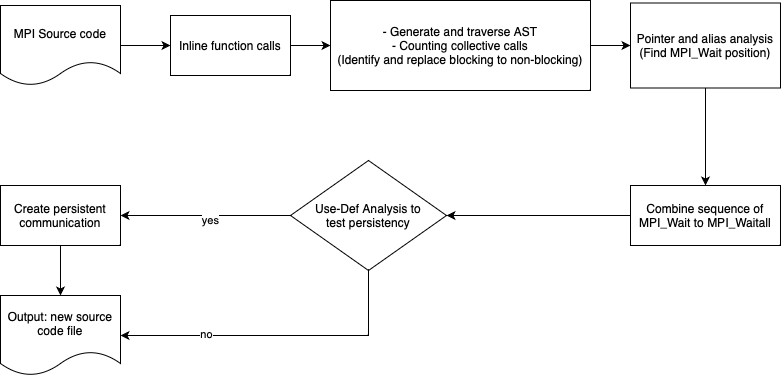
\includegraphics[width=0.7\textwidth]{pictures/petal_collective-workflow.png}
    \caption{The Petal transformation framework for collective communications. Adapted from \cite{ahmed_transforming_2017}}
    \label{fig:petal-collective-workflow}
\end{figure}

After inlining all the function calls, within each block, calls to blocking collectives will be counted. 
The count is required in order to reuse the same request for communications on mutually exclusive paths and allocate the necessary number of \texttt{MPI\_Request} and status objects. 

Rose's built-in CodeThorn \cite{margaria_verification_2014} analysis tool offers methods for creating a data flow analysis (DFA) that counts and keeps track of the locations of MPI blocked functions. 

Once Petal has determined the total number of MPI calls, it allocates the necessary request and status objects in the form of two arrays at the beginning of the main function; one for \texttt{MPI\_Request} which is set to \texttt{MPI\_REQUEST\_NULL}, and the other for \texttt{MPI\_Status}. Finally, Petal transforms the blocking collective calls to non-blocking collective primitives. 

To this end, it changes the blocking function calls to the corresponding non-blocking function. In addition, it appends the \texttt{MPI\_Request} object to the argument list. The request handle is an element from the request array with the index subscript assigned by DFA.

The next step is to locate an area where \texttt{MPI\_Wait} can be inserted that provides sufficient communication-computation overlap. 
The more computation we can overlap with communication, the better we can hide costs associated with communication.
One or two references to message buffers are required as arguments for MPI communication calls. Because of this, Petal makes use of pointer alias analysis to identify code that adds dependencies.  
For each collective call that follows a collective MPI call, Petal collects read and write variables.

If the buffer or its aliases is among the write variables, then the statement is considered unsafe. 
The \texttt{MPI\_Wait} that concludes the collective call has to be inserted before it.

For a read variable, this requirement can be relaxed under certain conditions. If the buffer is used only for sending, a read does not introduce an unsafe dependency and the \texttt{MPI\_Wait} can be moved across it. However, if it is a receive buffer, then the read introduces a true dependency and the \texttt{MPI\_Wait} has to be inserted before it.

\lstinputlisting[language=C++, caption={Positions for \texttt{MPI\_Wait}}, label={lst:rank_blocking}]{listing/rank_blocking.cpp}

\break

Petal considers the fact that most collective operations involve two buffers in communication. 
In certain operations like \texttt{MPI\_Reduce} and \texttt{MPI\_Scatter}, one of the buffers only plays a role at the root process and is not involved in communication with other processes. 
In \texttt{MPI\_Reduce}, the receive buffer is significant only for the root rank, whereas in \texttt{MPI\_Scatter}, it is the send buffer. 
The reason why the \texttt{MPI\_Wait} call can be different for root and non-root processes root MPI is due to the difference in communication patterns and responsibilities between these two types of processes.
Root processes may need to wait for multiple communication operations to complete before proceeding. For example, if the root process is collecting data from non-root processes, it may need to wait for all the non-root processes to send their data before it can proceed with the data collection. 
Meanwhile, non-root processes typically perform a specific computation or send their results to the root process or processes usually have a simpler communication pattern, often involving a single ``send'' or ``receive'' operation.
Non-root processes usually have a simpler communication pattern, often involving a single ``send'' or ``receive'' operation.
\autoref{lst:rank_blocking} illustrates an example where the optimal placement of \texttt{MPI\_Wait} depends on whether the process is the root or not. 
Petal calculates the appropriate position for \texttt{MPI\_Wait} for both the root rank and other ranks. 
If the computed positions are the same, Petal simply uses \texttt{MPI\_Wait}. However, if the positions differ, it inserts \texttt{MPI\_Wait} at both positions, protected by a condition that checks the rank against the MPI process. 
This allows non-root ranks to proceed with computation in certain cases, while the root rank must wait for the completion of scatter or reduce, as depicted in \autoref{lst:rank_non-blocking}.

\lstinputlisting[language=C++, caption={Transformed non-blocking code}, label={lst:rank_non-blocking}]{listing/rank_non-blocking.cpp}

In case, if a function call cannot be inlined, due to it its implementation not being available, Petal analyzes the call's arguments. 
If one of them relates to the message buffer in question, Petal treats this call as unsafe. 
Otherwise, the call is considered independent and can be overlapped safely with communication. 
The exception to this rule are calls to other MPI functions. Since MPI is a standard specification, Petal understands its API and arguments. 
Petal has stored information for each MPI function in arrays and whether an argument is read or written. 
Using this information as part of the message buffer analysis, Petal decides whether concurrent communications are feasible or not. 
If there is no dependency between all the communication message buffers, (i.e., only sending buffers can be identical), communication calls can overlap as well. 

\lstinputlisting[language=C++, caption={Blocking concurrent communication.}, label={lst:blocking_collective_cc}]{listing/collective_cc_blocking.cpp}

\autoref{lst:blocking_collective_cc} shows an example of this case. 
By looking at the message buffer of the three consecutive \texttt{MPI\_Bcast} for \texttt{foo}, \texttt{bar}, \texttt{foobar}, Petal is able to detect that they are all distinct and hence can be safely overlapped. 
\autoref{lst:non-blocking_collective_cc} shows the transformation's output.

\lstinputlisting[language=C++, caption={Transformed non-blocking concurrent communication.}, label={lst:non-blocking_collective_cc}]{listing/collective_cc_non-blocking.cpp}

Petal considers certain operations, such as \texttt{MPI\_Wtime}, \texttt{MP\_Barrier}, and \texttt{MPI\_Finalize}, to be special operations that cannot be overlapped with communication. 
Therefore, any communication that starts before calling these functions must be completed before executing these special operations. 
Petal includes \texttt{MP\_Wait} just before any of these special operations. 
To ensure that the \texttt{MPI\_Wait} is executed only when its corresponding nonblocking call is executed, Petal checks if the nonblocking initiation and wait for completion occur within the same scope. 
If they are in different scopes, Petal utilizes a flag that is set to true after initiating a nonblocking call. 
The corresponding \texttt{MPI\_Wait} is protected by a condition that checks if the flag is true. 
Once the wait operation is executed, the flag is reset. This ensures that the wait operation is executed only if the initiation call has been executed.

After locating every position for \texttt{MPI\_Wait}, Petal checks to see whether they can all be combined into one position. 
If there are no other active communications, Petal replaces each individual call that uses a series of request objects in a multiple wait call with a single 
\texttt{MPI\_Waitall} call. By comparing the subscript values of the requests in the set with the wait positions, Petal makes sure the requests are consecutive. 
Petal determines if there is at least one current communication with a different wait position and decides to insert each wait call separately if the difference between the maximum and minimum subscript values plus one does not equal the number of identified wait calls.

\autoref{collective_blocking} shows the code for solving $A \cdot x = b$ using the conjugate gradient method [source]. \autoref{collective_non-blocking} then illustrates how Petal transformed this code to its non-blocking version.
After inlining and counting collective calls, Petal creates corresponding arrays \texttt{reqs[2], flags[2]} and \texttt{stats[2]} in order to keep track of states for the calls. 

Petal detected that the arguments of \texttt{MPI\_Allgather} in line 14 are independent from the arguments of \texttt{SolvePrecondMatrix}, \texttt{ComputeVectorDotProduct} and the array \texttt{Bloc\_Delta1}. As a result, its \texttt{MPI\_Wait} with corresponding buffer can be placed at the end of the loop.
This collective call is also separate from collecting \texttt{Delta1} as well.
So that, its \texttt{MPI\_Wait} with corresponding buffers can be placed at the end of the loop.

No other independent processing is identified because an argument to the \texttt{MPI\_Iallreduce} message is used immediately after the call. 
The receive buffer in this call is represented by \texttt{\&Delta1}. 
Since Line 18's computation reads from \texttt{Delta1}, it cannot begin before \texttt{Delta1} has been computed.

\lstinputlisting[language=C++, caption={Example with collective blocking communications}, label={collective_blocking}]{listing/collective_blocking.cpp}

\lstinputlisting[language=C++, caption={Transformed non-blocking collective version}, label={collective_non-blocking}]{listing/collective_non-blocking.cpp}


\section{Experimental Evaluation}
This section will present some findings from the initial assessment of utilizing Petal and its impact on the overall performance of the application. Multiple tests were conducted on various environments.
\subsection{Point-to-point Communications}

Ahmed et al. \cite{hoefler_case_2007} benchmarked a series of tests, which were transformed using Petal tool, including 1D heat decomposition, 2D heat decomposition  \cite{ahmed_petal_2016}, and DT from the NAS NPB 3.3 \cite{noauthor_nas_nodate}. 
The performance of the transformed application was evaluated by varying the number of MPI processes. In the case of 1D heat, the number of MPI processes ranged from 6 to 200 tasks. 
For 2D heat and DT with classes W (Class W: workstation size - a 90's workstation; now likely too small) and A (standard test problems; ~4X size increase going from one class to the next), the number of MPI processors (NP) varied between 16 and 256. 
The results, depicted in \autoref{fig:p2p-benchmark}, demonstrate the execution time speedup 
$S = T_{\text{original}}/T_{\text{transformed}}$ achieved through the application of non-blocking transformation and the addition of persistent communication.
where $T_{\text{original}}$ is the the time needed to executed code before the transformation with Petal and $T_{\text{transformed}}$ is the execution time of the code after Petal substituted blocking communication with non-blocking or persistent one.
Analyzing the execution time of the original and transformed codes provides valuable information regarding the potential performance improvement achieved through the transformation. A ratio of $S = 1$ indicates no speedup. A ratio $S < 1$ implies that the transformed code performs worse, while a ratio of $S$ around 1 signifies a negligible performance gain.
The higher the value of $S$, the more performance gain can be achieved.\\

The experiments were conducted using the TACC Stampede System, which is a Dell Linux Cluster capable of processing 10 Petaflops (PF). 
The cluster consists of over 6400 Dell PowerEdge server nodes, each equipped with 32 GB of memory and 2 Intel Xeon E5 processors (Sandy Bridge, 8 cores). 
Additionally, the nodes are augmented with an Intel Xeon Phi Coprocessor (Knights Corner, 61 cores) using the MIC architecture.


\begin{figure}[!h]
    \centering
    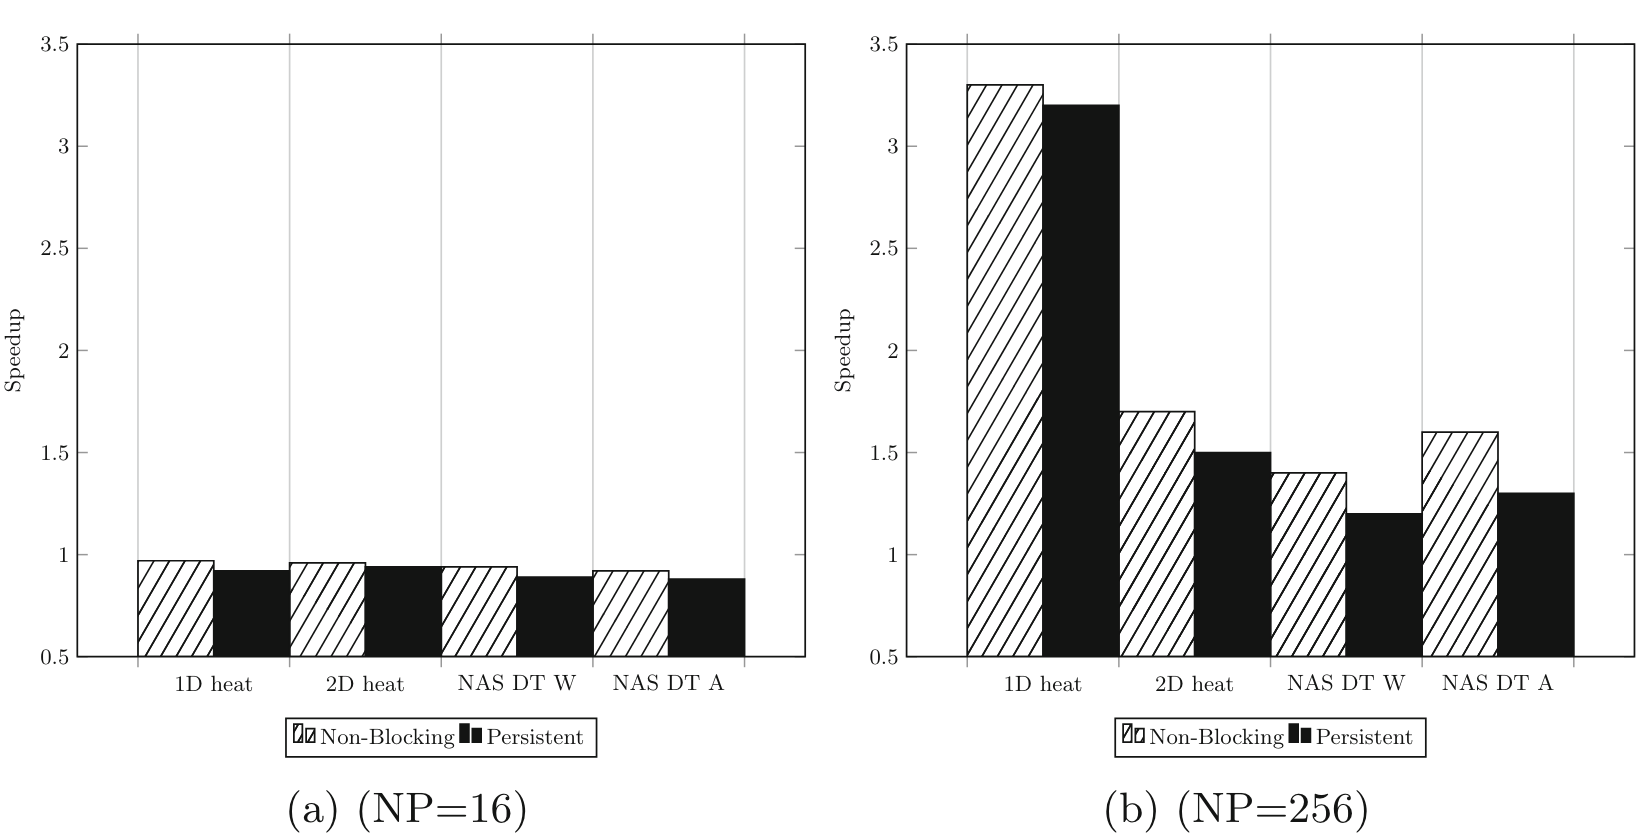
\includegraphics[width=\textwidth]{pictures/p2p-benchmark.png}
    \caption{Weak-scaling time speedup. \cite{ahmed_petal_2016}}
    \label{fig:p2p-benchmark}
\end{figure}
\autoref{fig:p2p-benchmark} provides a visual representation of the speedup achieved by the transformed code compared to the original code. The vertical axis represents the speedup, while the horizontal axis indicates the benchmarked problems.

When considering smaller programs and a smaller number of jobs, the speedup remains consistently below 1. This indicates that the benefit of non-blocking improvements is negligible and can sometimes even introduce overhead, resulting in worse performance.

However, significant performance improvements are observed with the non-blocking technique, with some cases showing increases of up to 30\%, such as in the NAS DT class A example with 256 processes. 
These improvements are consistently evident across all the transformed codes, showcasing their effectiveness as the problem size and the number of MPI tasks increase.
\subsection{Collective Communications}
Ahmed et al. \cite{ahmed_transforming_2017} conducted a performance comparison between the original code and the transformed code that employed nonblocking collectives.

The first test uses a C version of a benchmark code discussed by James Tullos \cite{Tullos_2014}. 
There is a code kernel consisting of three arrays, which are spread across multiple ranks. 
In this kernel, the first array is averaged, and the resulting value is utilized to make modifications to the second array. 
The minimum and maximum values in the second array are identified and employed, along with the sum of the first array, to modify the third array. 
Afterwards, the third array is reduced to a single sum that encompasses all ranks.\\
In the implementation of Ahmed \cite{ahmed_transforming_2017}, the kernel operates on three arrays \texttt{sub\_arr1}, \texttt{sub\_arr2} and \texttt{sub\_arr3} that are distributed across the processes. 
It uses \texttt{MPI\_Allreduce} to compute the average of the first array.
Using the average to compute new entries for the second array. 
The next step computes the global minimum and maximum values of the second array by two \texttt{MPI\_Allreduce} operations. (line 6-7)
The last step adds the average of the first array to all elements in the second array and uses the global min and max values to update the entries of the third array (line 9 - 12).
A last call to \texttt{MPI\_Allreduce} computes the sum of the third array (last line).

The number of MPI processes was varied  from 16 to 128, and tested with different message sizes, ranging from 16K to 524K with 16 processes, and from 65K to 4M with 128 processes.
\autoref{fig:intel-benchmark} demonstrates the execution time speedup ($S = T_{\text{original}}/T_{\text{transformed}}$) achieved through the application of non-blocking transformation with Petal.

Another benchmark was performed for conjugate gradient \autoref{collective_non-blocking}, which was discussed on Section \ref{sssec:collective_communication}. 
\autoref{fig:conj-benchmark} shows the speedup of transformed non-blocking version and non-blocking persistent version in comparison to application with blocking communications.

The tests were performed on a system with the following configuration:
LLNL cab cluster with 1,296 nodes with 16 core and 32GB memory each node, Intel Xeon E5-2670. 
The nodes are interconnected by InfiniBand in QDR mode. Openmpi-gnu-2.0.0 MPI with the default settings was applied for these tests.

\begin{figure}[!ht]
    \centering
    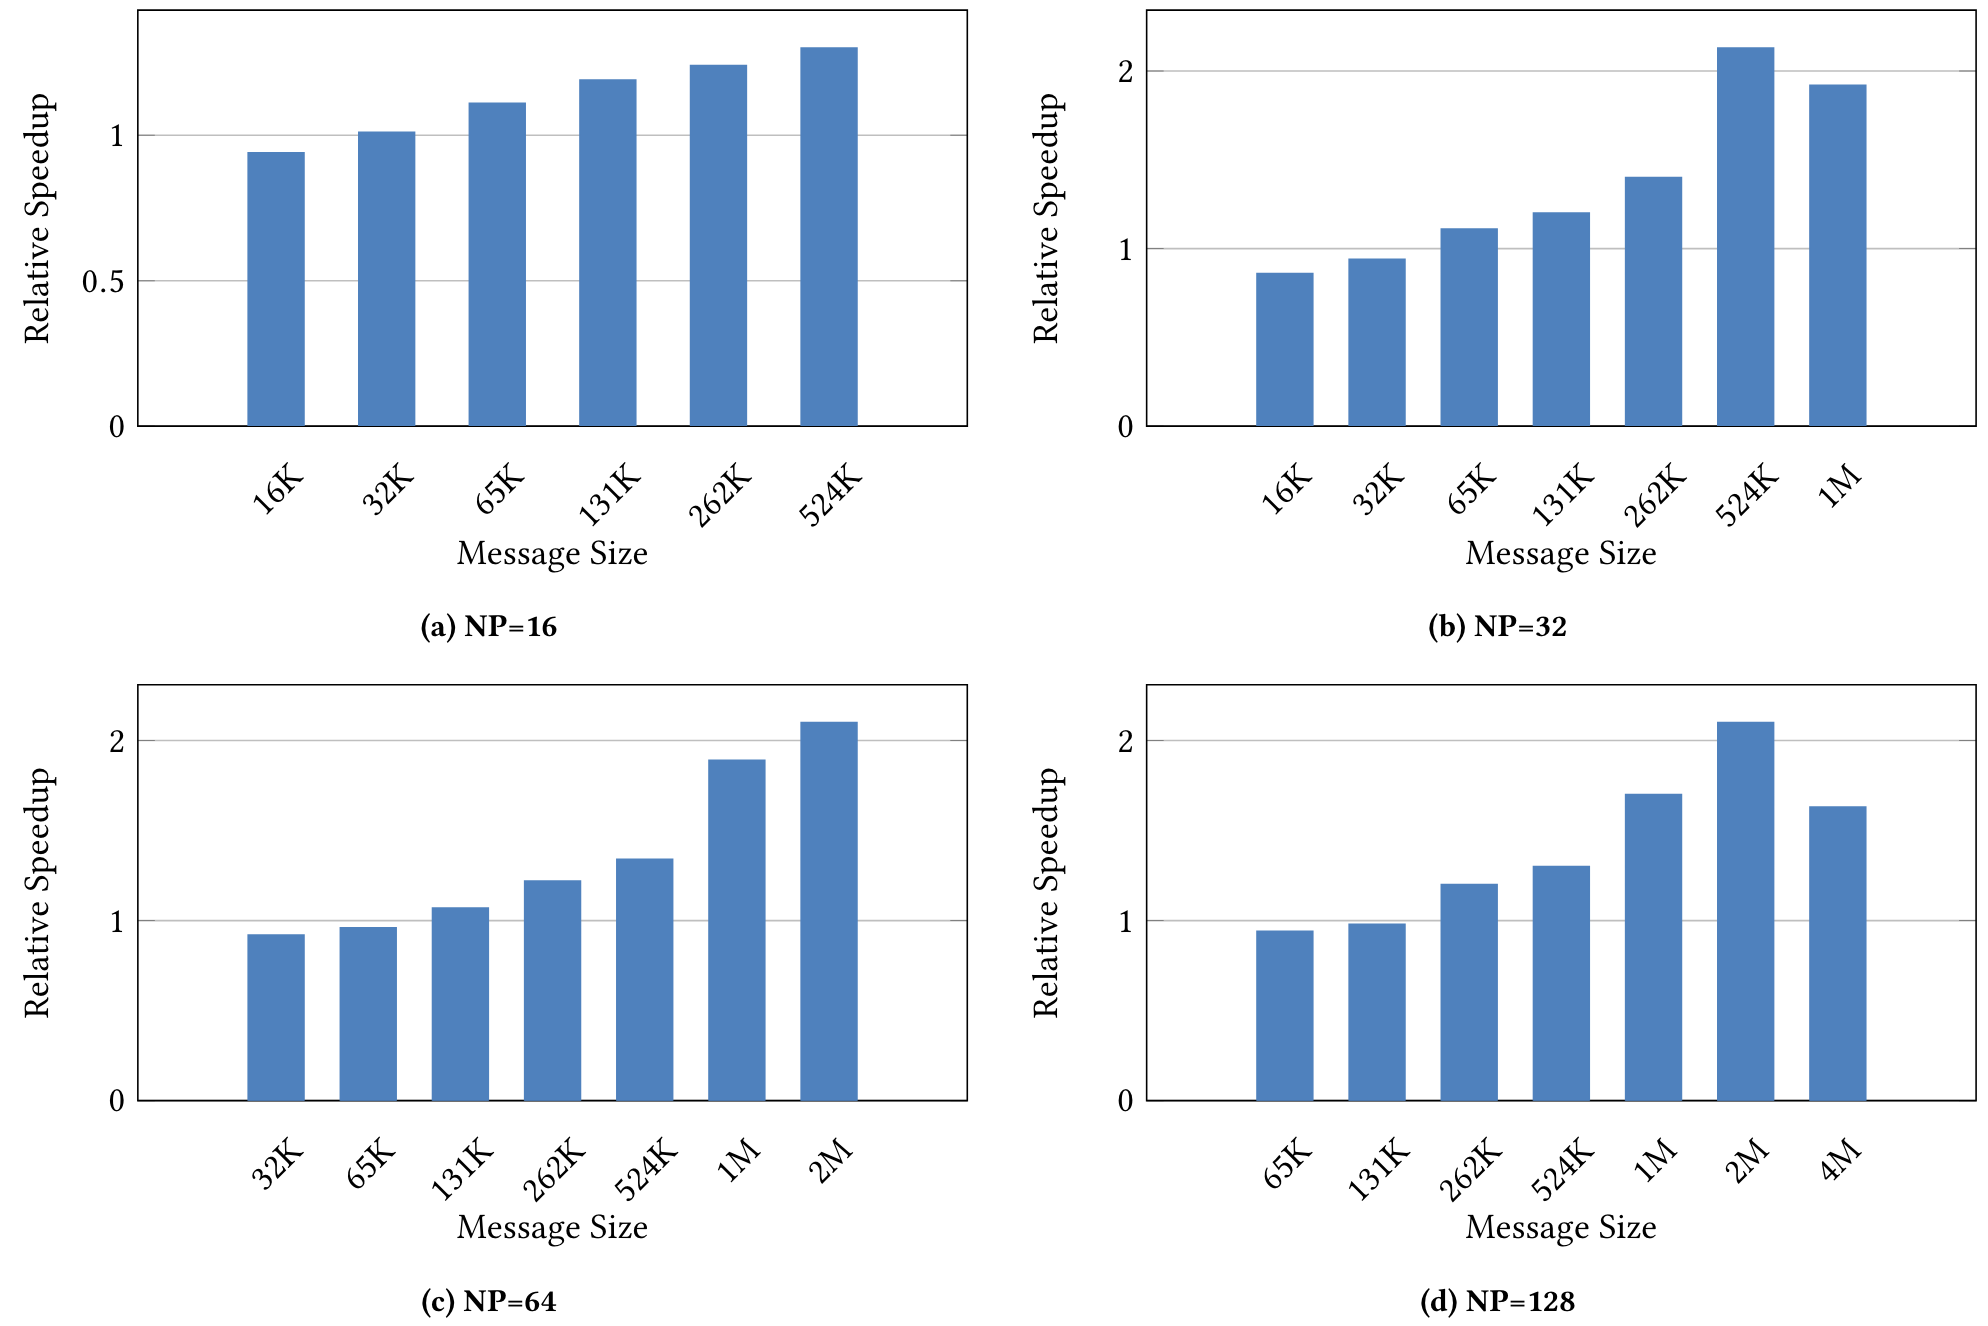
\includegraphics[width=\textwidth]{pictures/intel-benchmark.png}
    \caption{Weak-scaling for Intel benchmark. \cite{ahmed_transforming_2017}}
    \label{fig:intel-benchmark}
\end{figure}

\autoref{fig:intel-benchmark} illustrates the compwarative acceleration achieved by the nonblocking version in relation to the original code.
When utilizing 32 processes, enhancements are observed for message sizes exceeding 32K.
However, as the number of processes increases, the message threshold rises to 64K, 131K, and 262K, respectively, before the positive impact of nonblocking collectives becomes evident.
This phenomenon may be attributed to the relatively brief duration of overlapped computation compared to communication.
Under optimal circumstances, the nonblocking primitives achieve a twofold speedup compared to their corresponding blocking counterparts.
One of the potential factors contributing to this behavior is the utilization of cache.

\begin{figure}[!h]
    \centering
    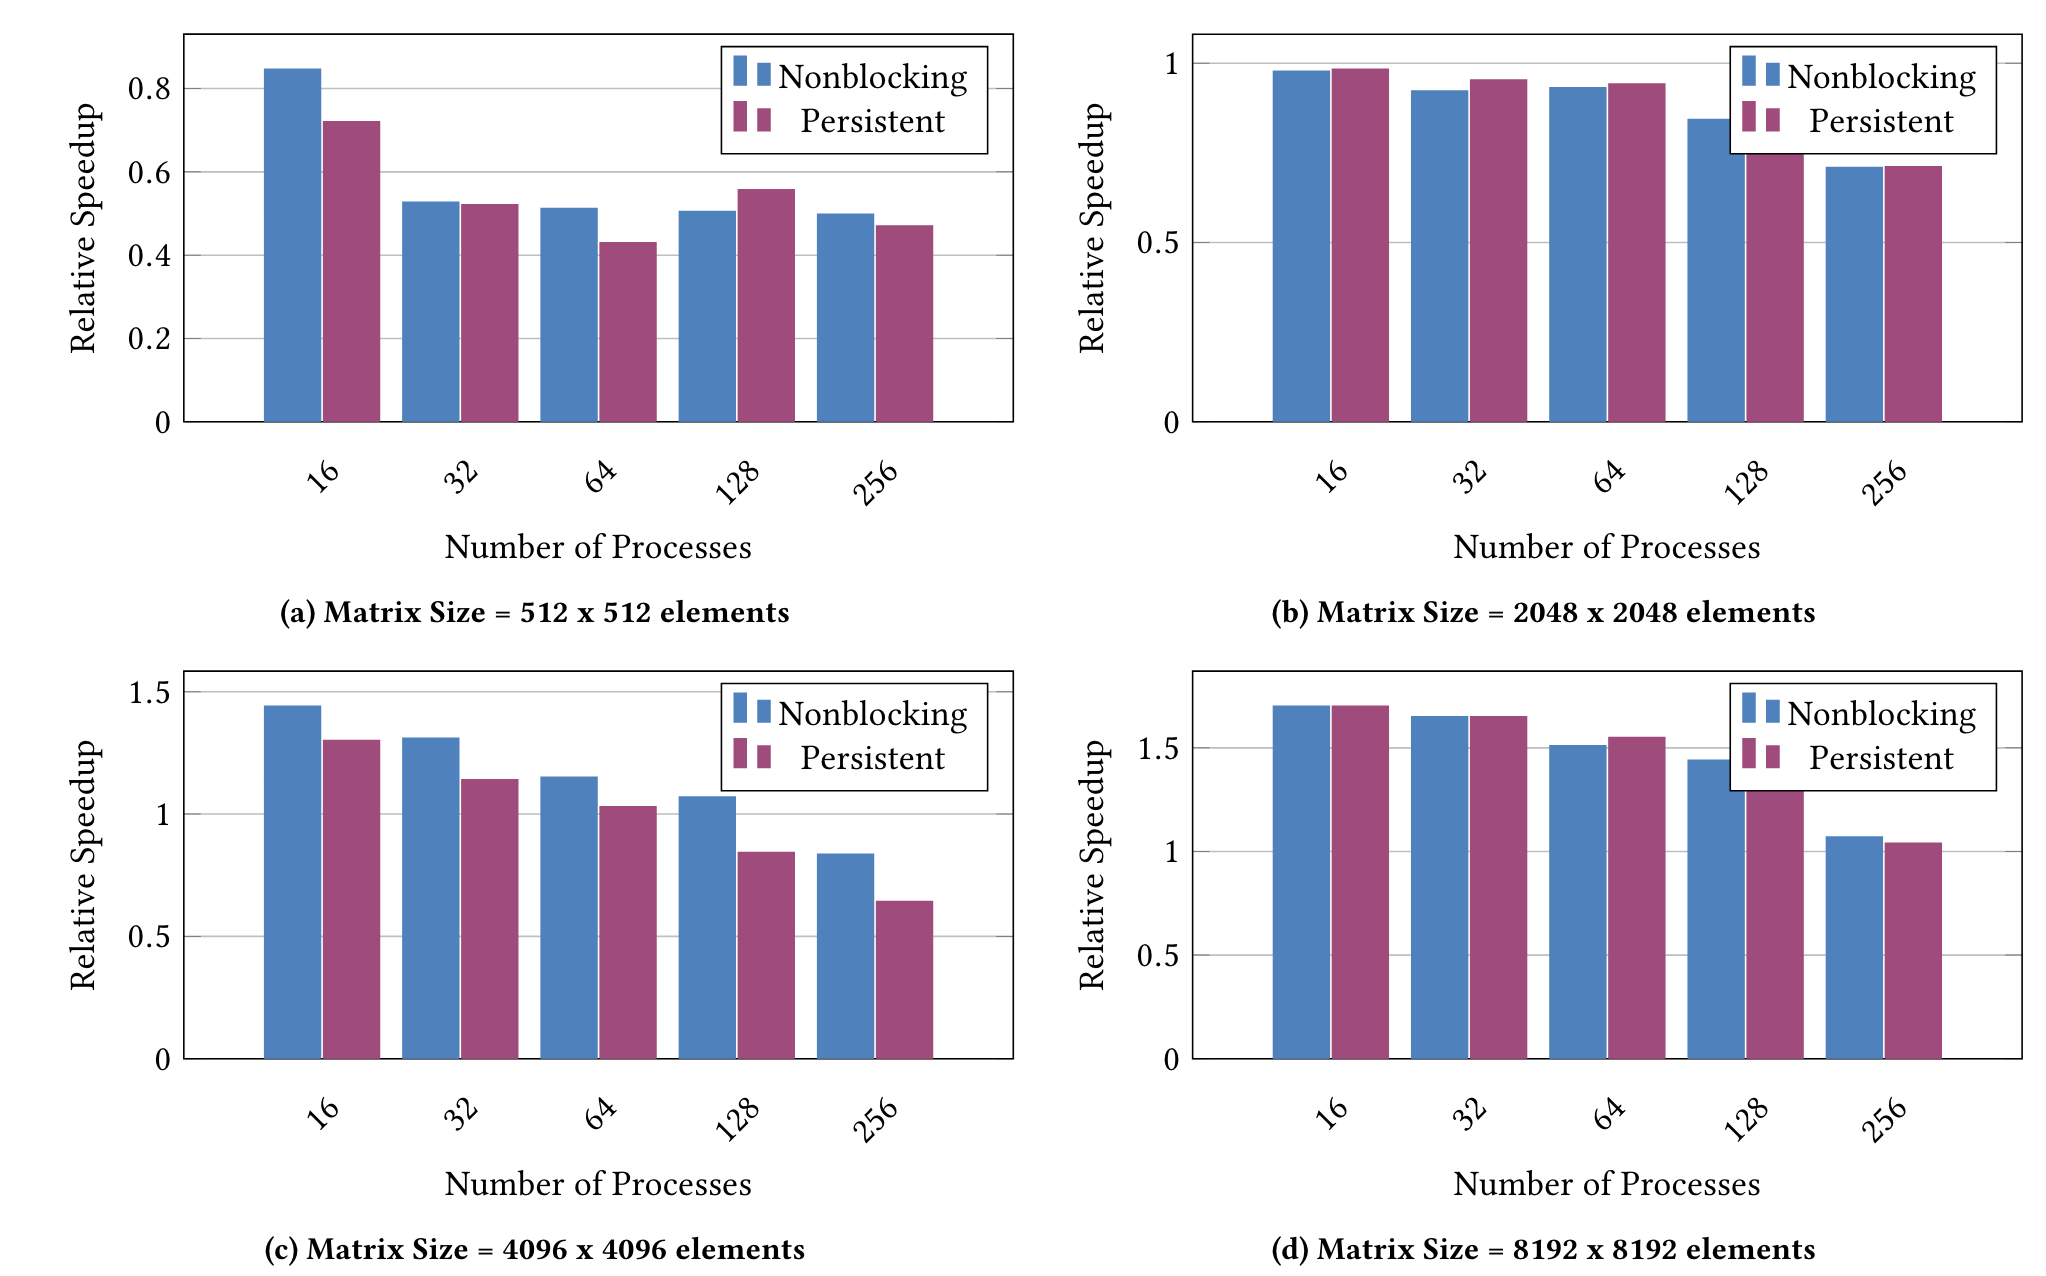
\includegraphics[width=\textwidth]{pictures/conj-benchmark.png}
    \caption{Weak-scaling for conjugate gradient benchmark.}
    \label{fig:conj-benchmark}
\end{figure}

For the conjugate problem \autoref{fig:conj-benchmark}, as the problem size increases, it becomes evident that the nonblocking version outperforms the blocking version. 
Nevertheless, with a higher number of processes, the benefits of using nonblocking operations diminish. 
This is primarily due to a reduction in the number of elements exchanged as the process count rises. 
Moreover, when dealing with extremely large matrix sizes, the conjugate gradient code for blocking collectives failed to complete within the allocated time on the machine, whereas the nonblocking version successfully finished. 
Ahmed et al. also implemented a transformation to persistent communication, which was not further explained in this paper. However, according to Ahmed et al., these transformations did not obtain any speedup improvement over its nonblocking counterparts.




\section{Discussion}
While Petal demonstrates its effectiveness in accurately identifying unsafe access to message buffers, there are limitations to its analysis in two specific scenarios. 
Firstly, it treats any access to a portion of an array as an access to the entire array. 
This means that even if only the first 10 elements of a 100-element array are sent via MPI, an assignment to the 20th element, located elsewhere and safe to use, will be deemed unsafe. 
Secondly, the Steensgaard algorithm \cite{steensgaard_points-analysis_1996} considers an access to a struct member as an access to the entire struct. 
These situations may result in overly cautious placement of \texttt{MPI\_Wait} in certain applications. 

At present, Petal lacks the ability to consolidate consecutive \texttt{MPI\_Wait} calls into a single \texttt{MPI\_Waitall} call when they occur within different code blocks, such as separate branches of an if statement. 
This limitation arises from the fact that the \texttt{MPI\_Isend}/\texttt{MPI\_Irecv} calls associated with each \texttt{MPI\_Wait} may originate from distinct sections of the code. 
It is desirable to discover an alternative approach, devoid of flags and if-statements, that preserves the code's semantics while enabling the utilization of \texttt{MPI\_Waitall} efficiently.

In a study conducted by Hadia \cite{ahmed_petal_2016}, the investigation focused on the implementation of non-blocking and persistent communications in the open-source framework Open MPI. The researchers discovered that Open MPI optimizes its code by employing persistent requests and utilizing them whenever applicable. 
As a result, modifying the code of applications to use persistence is unlikely to yield significant performance improvements, as Open MPI already employs similar optimization techniques internally. 
The observed slowdown could potentially be attributed to the overhead incurred from checking the arguments in each iteration.

The concept of overlapping communication and computation code has captured the attention of numerous researchers due to its potential to significantly enhance performance when effectively implemented.
In their study, Preissl et al. \cite{preissl_using_2008} propose an approach that also uses and leverages the infrastructure of ROSE to automate the conversion of blocking MPI calls to nonblocking calls. Their method involves a combination of static and dynamic analysis to detect and classify inefficient communication patterns, specifically identifying the Send- and Receive Events involved. But the researchers of this research did not still perform any evaluation of their approach yet.

PLUTO \cite{noauthor_pluto_nodate} is a framework designed for automatically parallelizing and optimizing the locality of affine loop nests. It can be combined with ACDL \cite{frohn_adcl_2023}, an auto-tuning framework for blocking and non-blocking collective operations. In their work, Gabriel and Barigou \cite{barigou_maximizing_2017} were able to transform parallel application software automatically using these frameworks, resulting in a performance improvement ranging from 32\% to 43\% compared to the version that utilized blocking communication operations. 
Additionally, they achieved a relative overlap ratio (ROR) of up to 95\% of the maximum theoretical communication-computation overlap identified for each scenario.

Bronevetsky et al. \cite{lumsdaine_compiled_2013} propose CoMPI, a compiler-driven tool aimed at enhancing the scalability of legacy MPI applications for Exascale systems. The primary objective of CoMPI is to enable incremental modifications that improve scalability. To achieve this, CoMPI introduces a set of source code annotations that provide insights into the usage of MPI in the applications. By leveraging compile-time and run-time analysis techniques, CoMPI identifies MPI ranks executing on the same node. This enables CoMPI to optimize communication by fusing send and receive operations and eliminating intermediate send and receive buffers. This optimization is achieved by replacing message serialization and deserialization loops with direct memory accesses. CoMPI specifically targets applications that explicitly perform data serialization and deserialization.

\section{Conclusions}

This paper presents and evaluates Petal, a compiler analysis tool designed to convert MPI blocking operations into their corresponding nonblocking versions. 
Petal's main objective is to identify instances where communication can be overlapped with independent work, thereby harnessing the benefits of nonblocking poin-to-point and collective routines introduced in MPI-3, ultimately enhancing application performance. 
To achieve this, Petal replaces blocking calls with their non-blocking counterparts and employs pointer and alias analysis to strategically insert \texttt{MPI\_Wait} statements in the appropriate locations. 
This allows for the overlapping of independent communications and/or computation tasks. 

The utilization of nonblocking collectives in certain cases has been shown to yield benefits for applications. 
This is particularly evident when dealing with sizable messages and when there is a sufficient amount of work available to overlap with communication tasks. 
Generally speaking, there were specific scenarios where the overlapping of communication and computation was feasible. 
These instances of value are expected to be further amplified in the future, especially for applications that have a higher percentage of work dedicated to communication and operate on systems with MPIs that offer robust progress and blocking communication completion (the optimal conditions for overlapping communication and computation).
Additionally, networks with increased message-passing concurrency will also reap the rewards of code restructuring.



% Print references
% Add entries to "literature.bib"
\printbibliography

\end{document}